\chapter{Introduction}




\section{Background motivation and need for this survey study}


For autonomous vehicles traversing in real world environments, robust obstacle avoidance is a fundamental safety requirement. However, ensuring obstacle avoidance is complicated. We therefore wish to compute safe and optimal trajectories with respect to a cluttered environment. However, computing optimal trajectories through cluttered environments introduces additional computational complexity as the number of obstacles considered in the optimization increases. Advances in research have brought the quadrotor to a level of sophistication that is making it increasingly attractive
for a variety of commercial applications like surveying and delivery. In order for these applications to become a reality, we now need algorithms that can deal reliably with environments that are substantially more cluttered than a laboratory setting. The most successful algorithms put forward to enable quadrotors to avoid obstacles often require an exponential
increase in planning time with respect to the number of obstacles by, for example, introducing an integer variable for each face of obstacles in the environment. Most of these algorithms therefore start to perform poorly as the number of obstacles is increased beyond a modest handful of them.~\cite{mellinger2012mixed,schouwenaars2001mixed}.

For planning trajectories with obstacle avoidance in a
known environment, generally we used to add non-convex
constraints to an optimization for obstacle avoidance in order
to ensure that our trajectory remains outside the set of ob-
stacles. Such constraints prevent us from finding guarantees
of completeness or global optimality in our program. We
can avoid some of the problems of non-convex constraints
by adding a discrete component to optimization. So for that,
if we model the non-convex set of obstacle-free states as
union of finitely many convex regions, then we can perform
a mixed-integer convex optimization in which the integer
variables correspond to assignment of trajectory segments to
convex regions. But, the approach mentioned is not without
consequences, as even the addition of binary variables (con-
strained to either take values 0 or 1) makes the problem from
linear program into mixed-integer linear program, which is
known to be NP-complete (as it is both NP and NP-hard).
Earlier implementations typically used the faces of each
obstacle to define the convex safe regions, which was used
to encode obstacle avoidance for UAVs as a mixed integer
linear program (MILP) by~\cite{schouwenaars2001mixed,culligan2006online,hao2005differential,richardsco}.

Recently, it has been suggested that the challenges of
increasing obstacle density may be overcome by the novel
Iterative Regional Inflation by semidifinite programming
algorithm (IRIS) that segments space into obstacle-free
regions. Planning paths through this segmentation can be
accomplished using mixed-integer convex optimization, with
the complexity growing with the much more manageable
number of free-space segments instead of the number of
obstacle faces. Hence, it can produce trajectories in environ-
ments containing many more obstacles than was previously
demonstrated. Moreover the non-penetration constraint that
the algorithm enforces along the entire path promise better
performance with small obstacles than previous approaches
that rely on sampling. We hypothesized that it would be
possible to aggressively fly a small quadrotor through en-
vironments containing greater number of obstacles than
ever demonstrated before by leveraging IRIS, MISDPs, and model-based control approaches. This document presents experimental validation of this hypothesis and of the planning algorithm introduced in~\cite{deits2015efficient}. 

\section{Related Work}

A few planning algorithms have been successfully applied to planning for quadrotors in moderately crowded environments. The approach in~\cite{richter2013polynomial} consisted of running RRT* in the
entire space where the quadrotor might fly. The algorithm
only expanded the randomly-exploring tree with straight
paths in order to make its expansion more efficient. It there-
fore resulted in a piece-wise linear collision-free trajectory.
Finally, the algorithm computed a smooth trajectory using a
quadratic program between each node along the path returned
by RRT*. Although a very efficient approach, relying on
sampling of space in order to check for collisions makes it
potentially difficult to deal with very small obstacles like
the strings used in our experiment. ~\cite{mellinger2012mixed} demonstrated the use of mixed-integer quadratic programs in order to plan collision-free trajectories. In this particular work, the integer
variable enforced non-penetration by making sure that the
sampled location is on the collision-free side of at least one
of the faces of each obstacle. The approach worked well in
practice, but it suffered from having the number of integer
variables grow rapidly with the number of obstacles. The
technique once again cannot guarantee to generate collision-
free trajectories between sample points, unlike our presented
approach.

IRIS, the described choice of algorithm for convex segmentation
of free-space, has previously been used in the context of
collision-free footstep planning~\cite{deits2014convex}. In this application, the algorithm generated obstacle-free regions in the robot’s configuration space. A mixed-integer program was then used to assign steps to each regions while simultaneously optimizing the pose of the robot. ~\cite{deits2015efficient} then went on to demonstrate that
we could formulate the problem of planning minimum-snap
collision-free trajectories as a mixed-integer semidefinite
program by using the obstacles-free regions returned by IRIS
and by planning in differentially flat space. This document in
part aims to provide experimental demonstrations for these
results.

~\cite{mellinger2012trajectory} demonstrated a feedback controller for aggressive flight inspired by the work of Hoffmann et al.~\cite{hoffmann2008quadrotor}. In this approach,
an off-board controller computed the position and velocity
error of the quadrotor and an on-board attitude controller
converted the associated desired center of mass acceleration
to a desired attitude. Finally,~\cite{barry2012flying} used time-varying LQR to demonstrate an aircraft with rotating wings executing a knife-edge maneuver in order to fly between two poles without colliding with either of them. 


\section{Modelling and System Identification}
The proposed approach uses the differentially flat quadrotor model introduced
in~\cite{mellinger2011minimum} and also used by others~\cite{richter2013polynomial}. Generally, a system is said to be flat if there exists a set of output, in equal number to
the number of inputs, such that all the states of the system
can be computed from these outputs (without integration).
In our quadrotor model, the flat outputs are $x, y, z$, position and yaw.

\begin{figure}[t]
	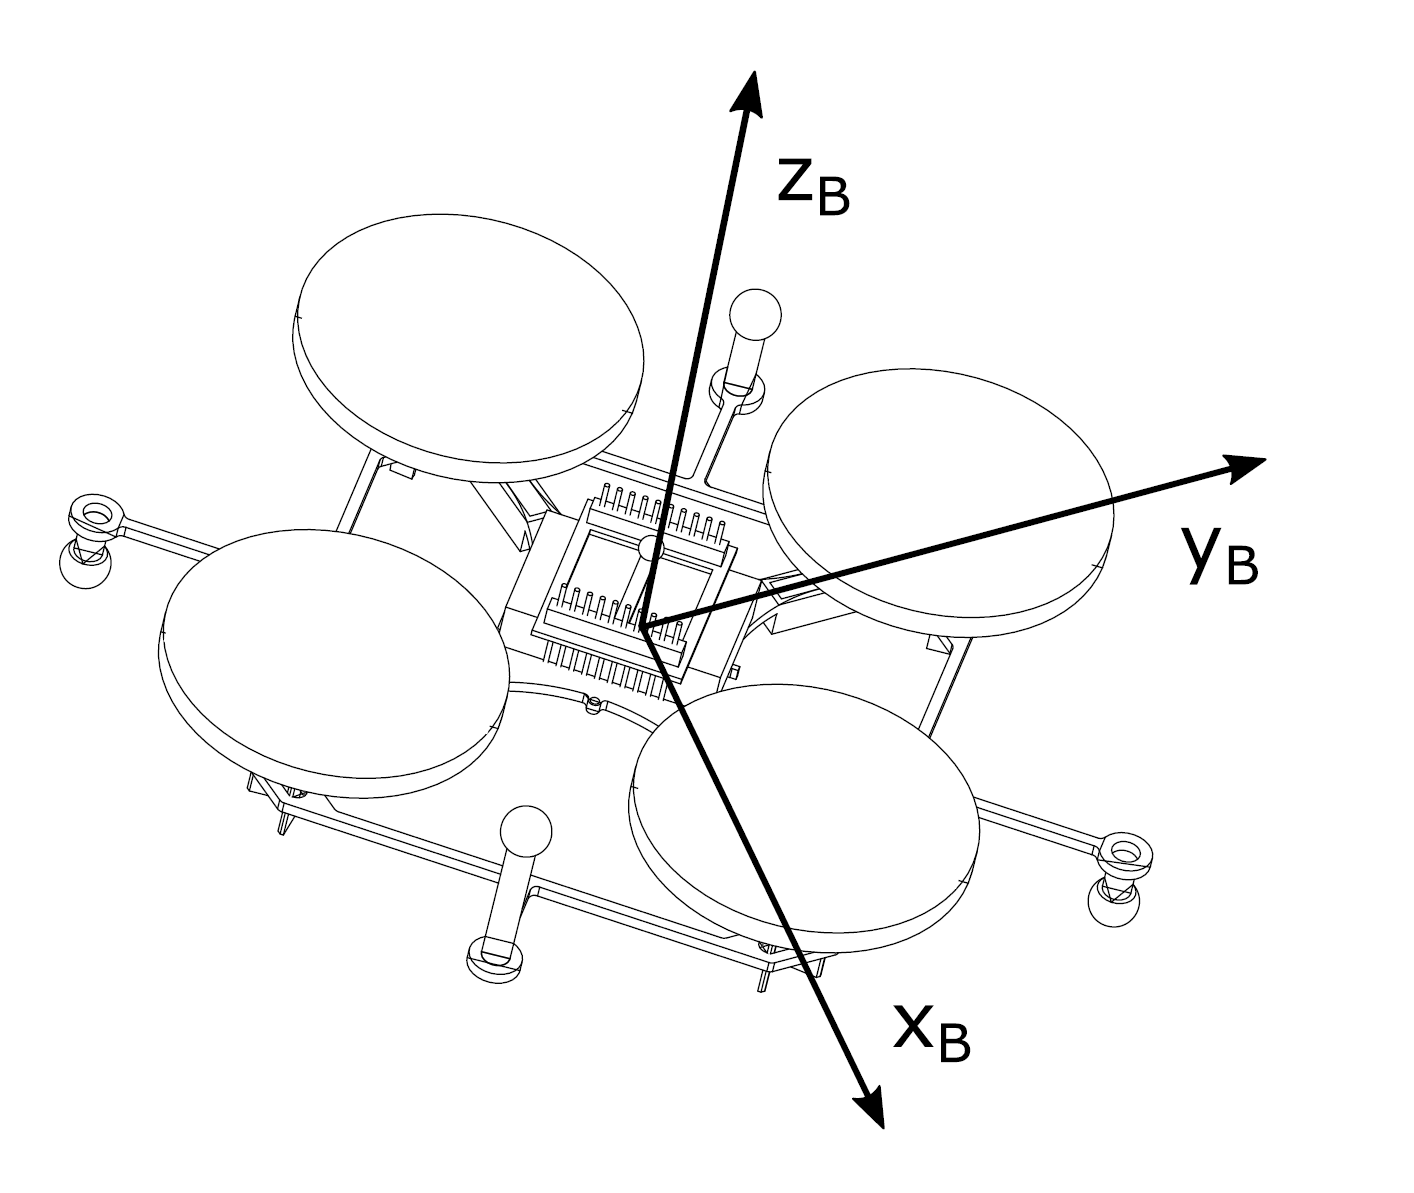
\includegraphics[width=0.9\linewidth]{img_crazyfly}
	\centering
	\caption{\label{fig: img_crazyfly}Model of the quadrotor used, the Crazyflie Nano
		Quadcopter, and the body frame used in the differentially flat
		model. $\boldsymbol{z_{B}}$ points in the same direction as propellers at all the time.}
\end{figure}
The model used in the study consists of a single floating rigid body and four
inputs. We define the inputs as the square of the angular velocities $\omega^2$ of the motors on the quadrotor. A spinning
propeller produces two forces on the quadrotor, namely lift
and drag. Those forces are directly proportional to $\omega^2$. Each
input $\omega_{i}^2$ can therefore be said to produce a certain linear
force $F_{i}$ on the center of mass as well as to create a moment $M_{i}$ according to\begin{equation} \label{eq: force_init}
F_{i} = k_{f}\omega_{i}^2,
\end{equation}\begin{equation} \label{eq: moment_init}
M_{i} = k_{m}\omega_{i}^2.
\end{equation}

We can then write the dynamics of the quadrotor:\begin{equation} \label{eq: dynamics_1}
m\ddot{r} = mg\boldsymbol{z_{w}} + (\sum_{i=1}^{4}F_{i})\boldsymbol{z_{b}},
\end{equation}\begin{equation} \label{eq: dynamics_2}
\boldsymbol{\dot{\omega}} = I_{}^{-1}(-\boldsymbol{\omega} \times I\boldsymbol{\omega} + W),
\end{equation}\begin{equation} \label{eq: dynamics_3}
W = \begin{bmatrix}
0 & k_{f}L & 0  & -k_{f}L \\ 
-k_{f}L & 0 & k_{f}L  &  0\\ 
k_m & -k_m & k_m & -k_m
\end{bmatrix}\begin{bmatrix}
\omega_{1}^2\\ 
\omega_{2}^2\\ 
\omega_{3}^2\\ 
\omega_{4}^2\\
\end{bmatrix},
\end{equation}where $m$ is the mass of the quadrotor, $\ddot{r}$ is the acceleration of its center of mass, $\boldsymbol{z_w}$ is a unit vector in the direction of gravity, $\boldsymbol{z_b}$ is a unit vector pointing in the same direction as the propellers (in the world frame), $I$ is the inertia matrix of the quadrotor, $L$ is the distance between each propeller and the center of mass of the quadrotor, and $\boldsymbol{\omega}$ is the angular velocity of the quadrotor in the body frame~\cite{richter2013polynomial}. 

We solve the problem of identifying the parameters of
this model with a two step approach. First, we directly or
semi-directly measure each parameter of the model with a
series of simple experiments. Second, we log flight data for a
series of maneuvers using a motion capture system, and use
an optimization-based algorithm to adjust those parameters. The $k_f$ parameter was identified by measuring the thrust
produced by the quadrotor placed upside-down on a scale and
fitting the corresponding parameter. The $k_m$ parameter can
be measured by slowly increasing a pair of opposite motors
(motors spinning in the same direction) and measuring the
resulting angular velocities using the on-board gyroscope. 

\section{Avoiding Obstacles}
The problem of obstacle avoidance is particularly chal-
lenging because the set of points outside a closed, bounded
obstacle is non-convex. As a result, we must generally add
non-convex constraints to an optimization in order to ensure
that our trajectory remains outside the set of obstacles. Such
constraints generally prevent us from finding guarantees of
completeness or global optimality in our program.~\cite{boyd2004convex}. We
can avoid some of the problems of non-convex constraints
by adding a discrete component to our optimization. If we model the non-convex set of obstacle-free states as the
union of finitely many convex regions, then we can perform
a mixed-integer convex optimization in which the integer
variables correspond to the assignment of trajectory seg-
ments to convex regions. This is not without consequences,
since even the addition of binary variables (that is, integer
variables constrained to take values of 0 or 1) turns linear
programming into mixed-{0, 1} linear programming, which
is known to be NP-complete.~\cite{karp2010reducibility}. However, excellent tools
for solving a variety of mixed-integer convex problems have
been developed in the past decade, and these tools can often
find globally optimal solutions very efficiently for mixed-
integer linear, quadratic, and conic problems~\cite{optimization2014gurobi,aps2014mosek,ilog2010cplex}. These tools also offer some anytime capability, since they can
be commanded to return a good feasible solution quickly or
to spend more time searching for a provably global optimum.

\par Earlier implementations of mixed-integer obstacle avoid-
ance have typically used the faces of the obstacles themselves
to define the convex safe regions. The requirement that a
point be outside all obstacles is converted to the requirement
that, for each obstacle, the point must be on the outside
of at least one face of that obstacle. For convex obstacles
these conditions are equivalent~\cite{mellinger2012mixed}. This approach has been successfully used to encode obstacle avoidance for UAVs as a
mixed integer linear program (MILP) by Schouwenaars~\cite{schouwenaars2001mixed}, Richards~\cite{richardsco}, Culligan~\cite{culligan2006online} and Hao~\cite{hao2005differential}. Mellinger et al.
add a quadratic cost function to turn the formulation into a
mixed-integer quadratic program (MIQP)~\cite{mellinger2012mixed}. However, this
approach requires separate integer variables for every face of
every obstacle, which causes the mixed-integer formulation
to become intractable with more than a handful of simple
obstacles.

Instead, IRIS, a greedy
tool for finding large convex regions of obstacle-free space is used here~\cite{deits2015computing}, to create a small number of convex regions to cover
all or part of the free space. These regions can be seeded
automatically based on heuristic methods or by an expert
human operator. We then need only one integer variable
for each region, rather than for each face of every obstacle.
We have previously demonstrated this approach for mixed-
integer footstep planning~\cite{deits2014footstep}, and it is also evident from the proofs shown in the following chapters that it
allows us to handle environments with tens or even hundreds
of obstacle faces.

\section{Safety of the Entire Trajectory}
Through the proposed approach, we have the ability to ensure that the
polynomial trajectory for the UAV is obstacle-free over its
entire length, rather than at a series of sample points. Existing
mixed-integer formulations have chosen only to enforce the
obstacle-avoidance constraint at a finite set of points~\cite{mellinger2012mixed,schouwenaars2001mixed,richards2002aircraft}. \begin{figure}[t]
	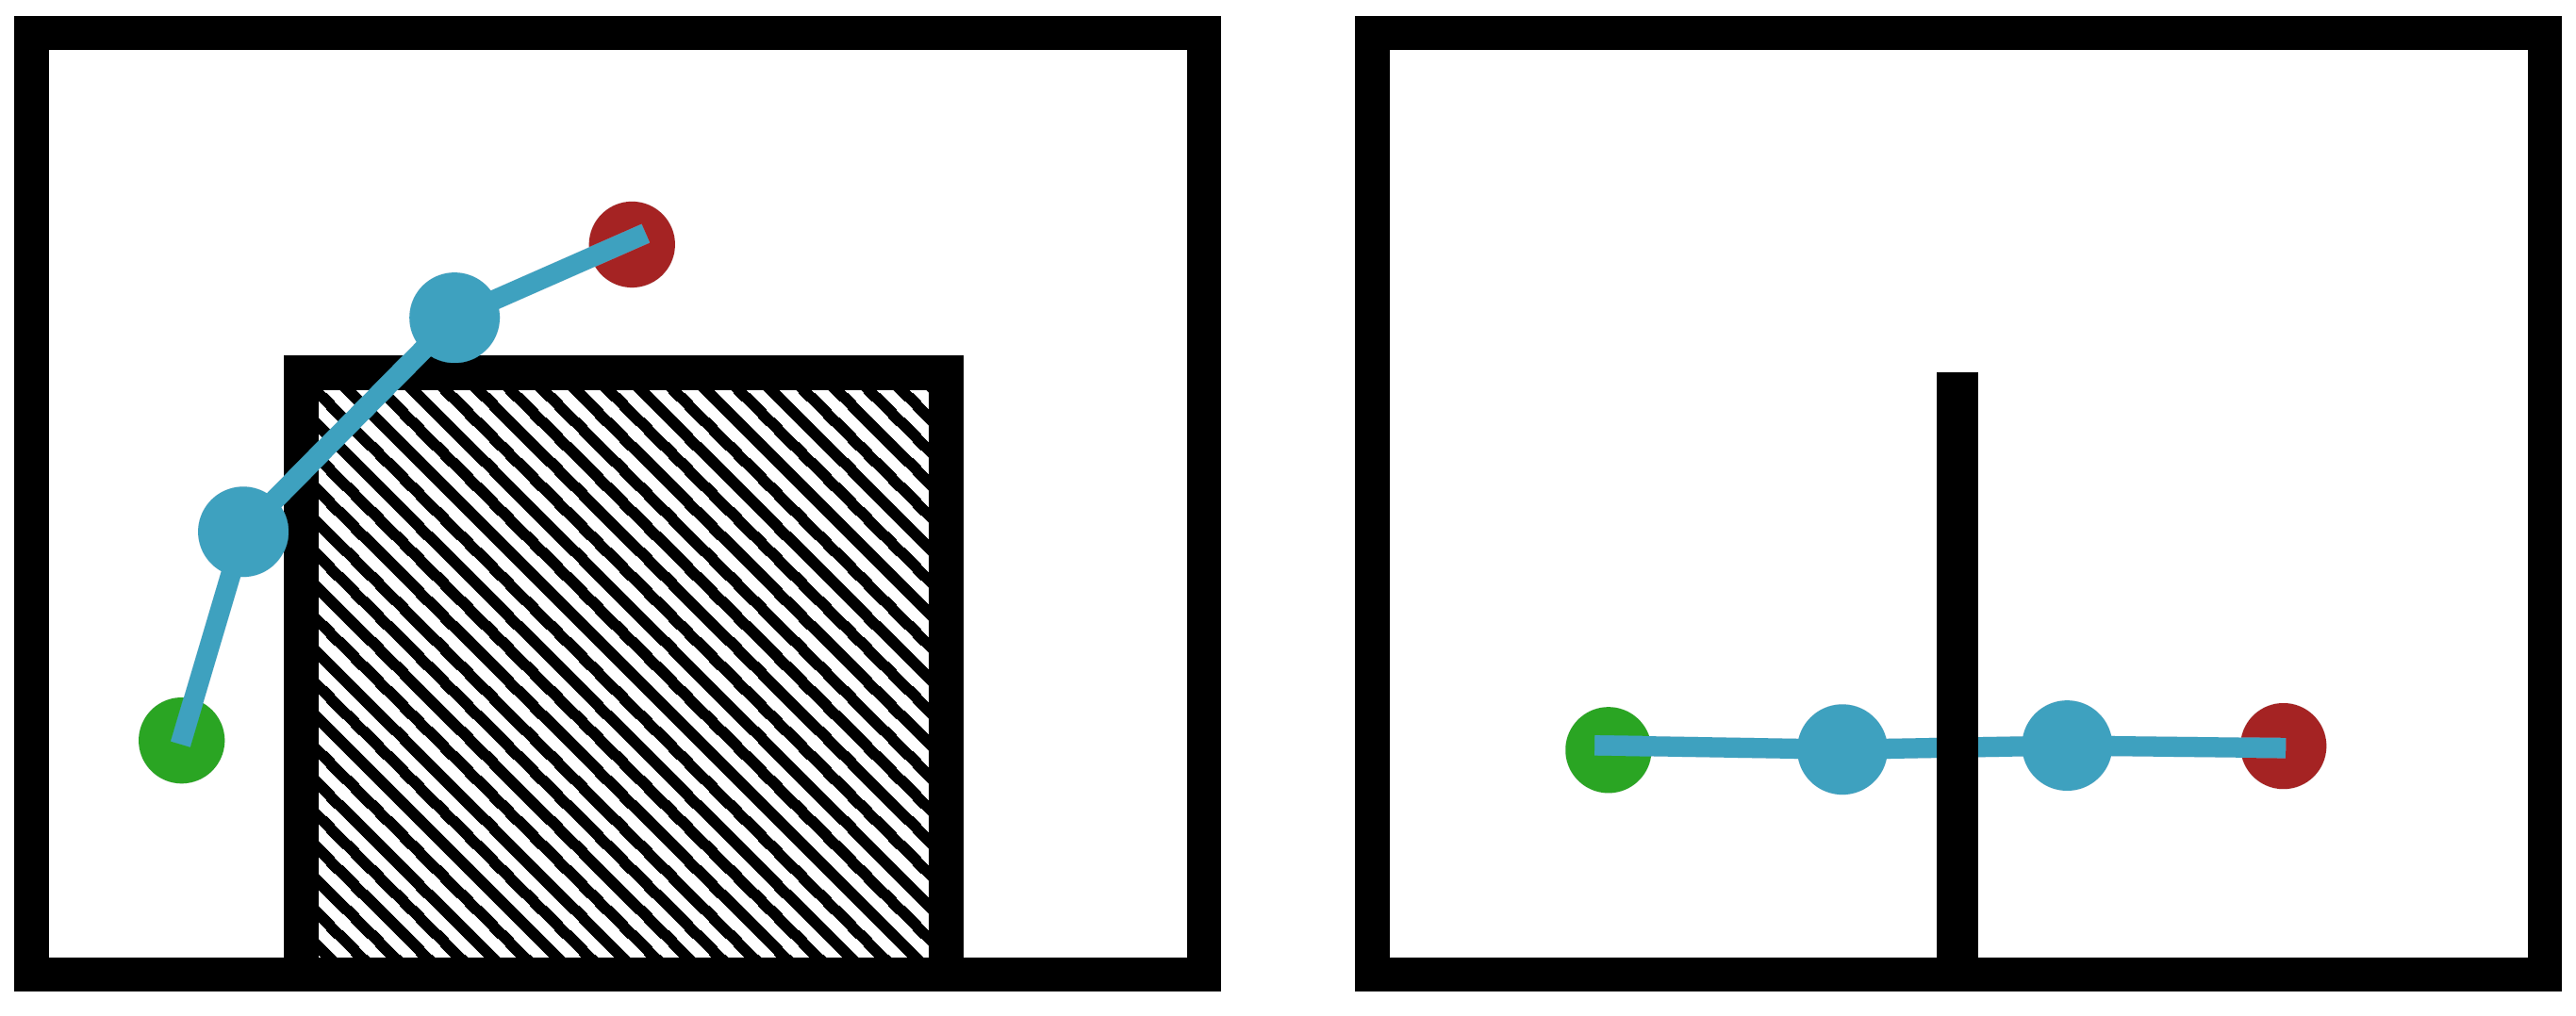
\includegraphics[width=0.9\linewidth]{fig_2}
	\centering
	\caption{\label{fig: cornercutting_1}A piecewise linear trajectory between two points, with obstacle
		avoidance enforced only at 4 points along each trajectory. The continuous
		trajectory through those points may cut corners or pass through thin
		obstacles.}
\end{figure}\begin{figure}[t]
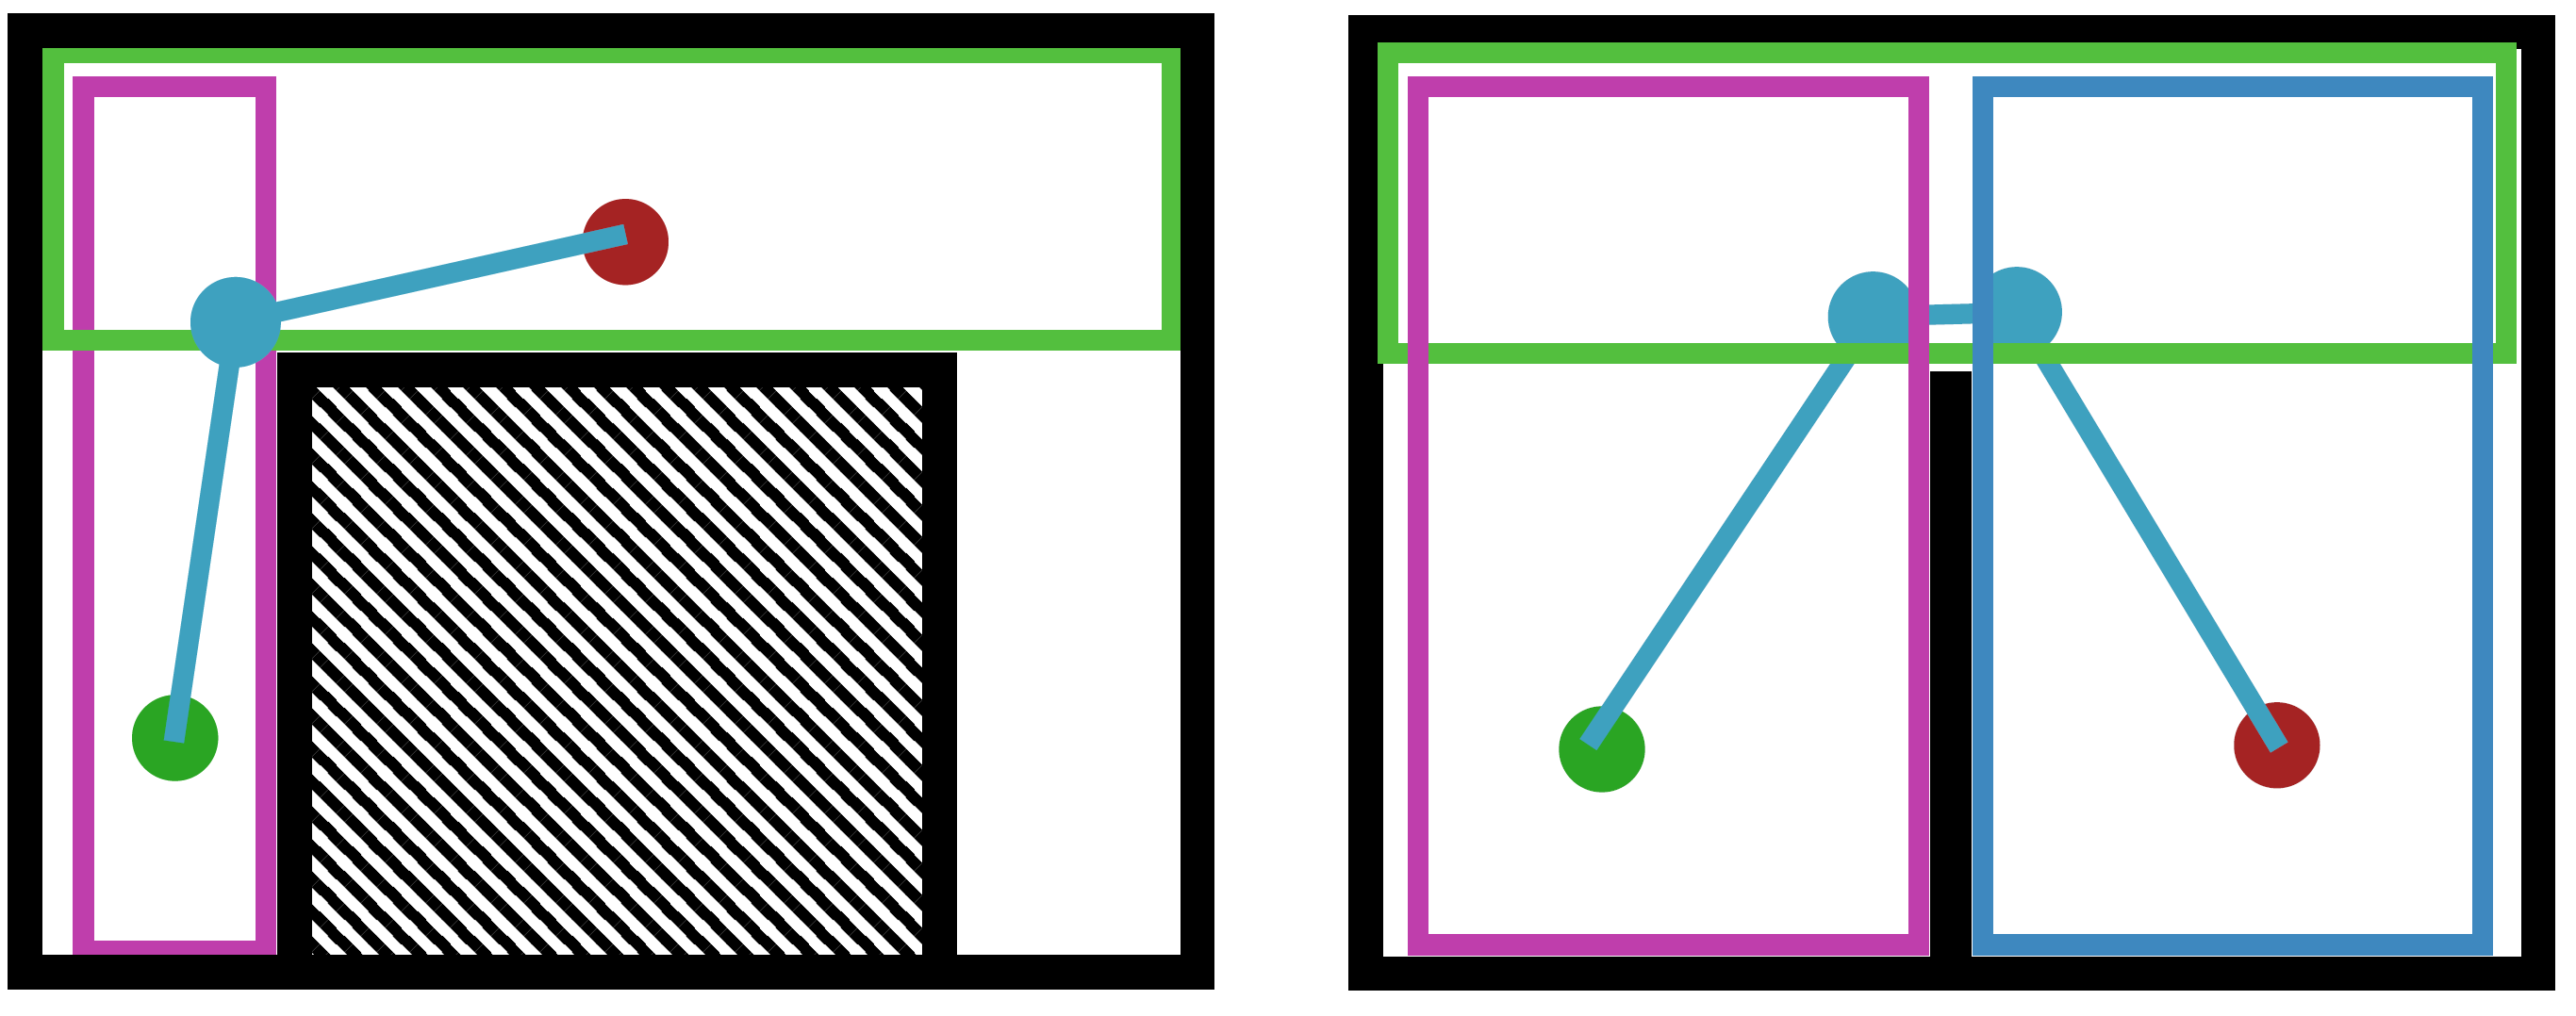
\includegraphics[width=0.9\linewidth]{fig_3}
\centering
\caption{\label{fig: cornercutting_2}A trajectory in which each linear segment is required to remain en-
	tirely within one of the convex obstacle-free regions indicated by the colored
	boxes. This requirement ensures that the entire trajectory is collision-free.}
\end{figure}This can result in the path between those sample
points cutting the corners of obstacles, or, more dangerously,
passing through very thin obstacles, as shown in Fig.~\ref{fig: cornercutting_1}. As noted by~\cite{bellingham2002coordination}, the severity of the corner cuts
can be reduced by increasing the number of sample points
and limiting the total distance between adjacent samples,
but this also increases the complexity of the optimization problem. Mellinger approaches this problem by requiring
that the bounding boxes of the UAV at adjacent sample points
must overlap~\cite{mellinger2012mixed}. This is sufficient to ensure that the UAV
never passes entirely through an obstacle, but it does not
necessarily prevent corner cutting. 

Representing the environment with convex safe regions
allows us to completely eliminate the cutting of corners. If
we treat the problem as one of assigning entire segments
of trajectories, rather than points, to the safe regions, then
we can create a fully collision-free trajectory. For piecewise
linear trajectories, this is simply a matter of ensuring that, for
each linear segment, both endpoints must be contained within
the same convex safe region, as shown in Fig.~\ref{fig: cornercutting_2}. This decision weakens our claim of optimality, since it requires the
breakpoints between trajectory segments to occur in the inter-
section of two convex regions, but it results in a formulation
that can be solved exactly with mixed-integer programming.
We enforce the constraint that each polynomial lie within a
convex region using a sums-of-squares (SOS) approach. In
this way, collision-free trajectories can be generated using
piecewise polynomials of arbitrary degree. Here we show
that, for trajectory segments defined by polynomials, we can
exactly enforce the constraint that each segment lies inside
a convex region by solving a small semi-definite program(SDP).


These polytopes, generated from IRIS must be given as an ordered union of only
pairwise adjacent sets, but the trajectories are guaranteed to
be contained within the polytopes by construction. Since the polytopes must be pairwise adjacent, they must be laid out
along a single path from start to goal by some other planning
procedure, and the resulting trajectories may not leave this
path. On the other hand, by performing our mixed-integer
optimization, we are able to explore arbitrarily connected
polytopes which may admit many different possible paths
through them.





